% =========================================================================
% manuscript.tex — live compile target (Overleaf-ready with references.bib)
% Sections 2-4 ported from paper/manuscript.md; every number traces to
% results/exp4_protocol_output.txt. Section 1: para 1 in place, 2-6 TODO (FL).
% Section 5: TODO (FL, per OUTLINE.md scaffold).
% =========================================================================
\documentclass[11pt]{article}

\usepackage[margin=1in]{geometry}
\usepackage[utf8]{inputenc}
\usepackage[T1]{fontenc}
\usepackage{amsmath, amssymb, amsthm}
\usepackage{booktabs}
\usepackage{graphicx}
\usepackage{natbib}
\usepackage[running]{lineno}
\usepackage{setspace}
\usepackage[hidelinks]{hyperref}

\doublespacing
\linenumbers

\newtheorem{proposition}{Proposition}

\newcommand{\dalpha}{\ensuremath{\Delta\alpha}}
\newcommand{\repo}{\url{https://github.com/francislinlfh-lgtm/Aspire-Project}}

\title{[TITLE --- see paper/OUTLINE.md shortlist]}
\author{Francis Lin\\{\small [Affiliation]}\\{\small \texttt{[email]}}}
\date{}

\begin{document}
\maketitle

\begin{abstract}
\noindent [Abstract --- written last. Must contain: \dalpha{} with CI; held-out
CV result; the T2 predictive-check failure.]

\medskip
\noindent\textbf{Keywords:} perspective-taking; common ground; reference
resolution; cognitive aging; computational modeling; director task
\end{abstract}

% =========================================================================
\section{Introduction}\label{sec:intro}

Understanding another person often requires setting aside information that is
obvious from one's own perspective \citep{samuel2025}. The problem is clearest in
reference resolution, where a listener must work out which object a speaker
means. Suppose a speaker and a listener both see two candles, and a third,
smaller candle is visible only to the listener. When the speaker asks for ``the
small candle,'' the candle that is smallest in the listener's view cannot be the
intended referent --- the speaker does not know it exists. To interpret the
request correctly, the listener must weigh not only which object best fits the
description, but which objects the speaker can see at all. Yet listeners
sometimes look at, and occasionally reach for, the hidden candle anyway
\citep{keysar2000} --- the classic egocentric error.

The processes underlying such errors --- documented most extensively in the
``director task'' paradigm \citep{keysar2000} --- remain disputed.
Egocentric-anchoring accounts propose that listeners initially interpret an
utterance from their own perspective and only later, through an effortful
correction process, adjust toward the speaker's knowledge; errors arise when
that adjustment is incomplete or delayed \citep{keysar2000,epley2004}.
Early-integration accounts instead argue that common-ground information
constrains reference resolution from the earliest moments of processing, such
that listeners do not necessarily begin from a fully egocentric interpretation
\citep{hanna2003}. A third possibility is that listeners represent both
egocentric and common-ground interpretations concurrently, with behavior
reflecting their relative probabilistic weighting rather than a fixed sequence
of anchoring and correction \citep{heller2016}. These accounts can produce
similar final choices even though they imply different underlying computations,
making aggregate error rates insufficient for deciding among them. More
fundamentally, the director task itself has been criticized as potentially
confounding perspective-taking with selective attention and task demands,
leaving open whether an ``egocentric error'' uniquely identifies a failure to
use common ground at all \citep{rubiofernandez2017}.

Existing computational work has formalized perspective use, but the central
quantity --- how much weight the egocentric perspective actually receives ---
has never been estimated from interpretive choices. \citet{heller2016}
introduced a probabilistic mixture parameter governing the relative contribution
of egocentric and common-ground information, but used it to generate qualitative
predictions rather than estimating its value from data. \citet{mozuraitis2018}
subsequently examined which ranges of a related parameter reproduced
condition-level patterns in reference production, without trial-level likelihood
estimation, participant heterogeneity, or age dependence. Other neighboring
approaches have modeled common ground as an inferred latent state evaluated
against offline judgments \citep{rubiofernandez2018} or fitted Rational Speech
Act parameters in a different communicative paradigm \citep{hawkins2021}. To our
knowledge, no previous study has estimated a comprehension-side
perspective-mixture weight from director-task choices using a participant-level
hierarchy, modeled that weight across adulthood, and evaluated the resulting
age-dependent account through held-out-participant prediction.

% TODO (FL): paragraphs 4-6 per paper/OUTLINE.md scaffold. NOTE the para-2 debt:
% para 6 MUST state plainly that this paper does not adjudicate the three
% accounts (explicit non-claim; Proposition 1) — para 2's setup requires it.

% =========================================================================
\section{Model}\label{sec:model}

\subsection{A choice-level projection of the domain-mixture account}\label{sec:projection}

\citet{heller2016} proposed that listeners resolve definite reference by weighing
two referential domains simultaneously: an egocentric domain (all objects the
listener can see) and a common-ground domain (objects visible to both
interlocutors). Their Equation~2 combines Bayesian reference resolution under
each domain with a weight $\alpha$ on the egocentric domain,
\begin{equation}\label{eq:heller}
  P(\mathit{obj} \mid \mathit{RE}) \;=\;
    \alpha\, P(\mathit{RE} \mid \mathit{obj}, d{=}e)\,P(\mathit{obj} \mid d{=}e)
    \;+\; (1-\alpha)\, P(\mathit{RE} \mid \mathit{obj}, d{=}c)\,P(\mathit{obj} \mid d{=}c),
\end{equation}
where an $\alpha$ near 1 corresponds to egocentric interpretation and $\alpha$
near 0 to full common-ground restriction. In the original paper, $\alpha$ was
varied from 0 to 1 to generate qualitative predictions; it was not estimated
from data.

We fit a deliberately reduced projection of this model to choice data. On a
critical director-task trial, the display admits exactly one best egocentric
referent (a privileged competitor matching the instruction) and one best
common-ground referent (the intended target). With point-mass within-domain
resolution, the model reduces, per trial, to
\begin{equation}\label{eq:projection}
  P(\text{select competitor}) = \alpha, \qquad
  P(\text{select target}) = 1 - \alpha,
\end{equation}
under a probability-matching response rule. This projection discards three
components of the full account --- graded, production-normed referring-expression
likelihoods; a ground-status prior; and incremental (partial-expression)
evaluation --- and therefore estimates $\alpha$ only at the level of final
choices.

\subsection{Hierarchy}\label{sec:hierarchy}

Participants vary. We model participant $i$'s weight as
\begin{equation}\label{eq:hierarchy}
  \alpha_i \sim \mathrm{Beta}\!\big(\mu(\mathrm{age}_i)\,\kappa,\;
    (1-\mu(\mathrm{age}_i))\,\kappa\big), \qquad
  e_i \sim \mathrm{Binomial}(n_i, \alpha_i),
\end{equation}
yielding an exact Beta--Binomial marginal likelihood. The primary age model is
logit-quadratic,
\begin{equation}\label{eq:curve}
  \operatorname{logit} \mu(\mathrm{age}) = \beta_0 + \beta_1 z + \beta_2 z^2,
  \qquad z = (\mathrm{age} - 53)/10;
\end{equation}
the comparator is the fitted constant-$\alpha$ model $(\alpha_0, \kappa)$. The
primary estimand is $\dalpha = \alpha(75) - \alpha(25)$.

\subsection{Response-rule conditionality}\label{sec:equivalence}

\begin{proposition}\label{prop:equivalence}
For two-alternative trials with point-mass domains, the probability-matching
rule with weight $\alpha$ and an argmax-plus-lapse rule with lapse rate
$\varepsilon$ (lapses uniform over the two alternatives) induce identical
likelihoods for every possible dataset under the mapping
$\varepsilon = 2\alpha$.
\end{proposition}

\begin{proof}
Under matching, $P(\text{competitor}) = \alpha$. Under argmax-plus-lapse with
$\alpha < .5$, the argmax is the target, so
$P(\text{competitor}) = \varepsilon/2$. Setting $\varepsilon = 2\alpha$ equates
the trial likelihoods, hence all products of them.
\end{proof}

Consequently, choice data cannot distinguish ``egocentric weighting'' from
``lapsing'' at this level: every $\alpha$ reported below carries its dual
reading $\varepsilon = 2\alpha$, and all psychological interpretation is
explicitly conditional on the response rule. Process-level data (e.g., graded
fixation measures) are required to separate the readings; we return to this in
the Discussion.

% =========================================================================
\section{Method}\label{sec:method}

\subsection{Data}\label{sec:data}

We reanalyze the open dataset of \citet{bradford2023}
(\url{https://osf.io/2epsu/}), an eye-tracked computerized director task with a
community lifespan sample. Participants followed prerecorded instructions to
move objects in a $4 \times 4$ grid with occluded slots; on Listener-Only
(critical) trials the occluded object matched the instruction (e.g., the
smallest of three candles, hidden from the director), so correct interpretation
required the director's perspective; on Shared-Perspective (control) trials the
occluded object did not match. Each participant contributed 12 critical and 12
control trials. We model critical trials; the trial-level outcome is the
authors' EgocentricErrors coding (selection of the hidden competitor); other
errors ($\approx$1.2\% of trials) count as non-egocentric, so the likelihood
estimates egocentric-choice probability specifically.

\subsection{Cleaning, with verification against published anchors}\label{sec:cleaning}

Exact byte-duplicate rows were removed (48 rows from two participants whose
sessions were duplicated in the file); one participant absent from the
demographics file and one with $\mathrm{FSIQ4} < 70$ were excluded,
reconstructing the paper's analysis sample of $N = 264$ (ages 20--86), each
with exactly 12 critical trials. Two published anchors were reproduced before
any model contact: the analysis $N$ (264) and the mean per-participant
egocentric rate (10.23\%, matching the 10.23\% reported by
\citealp{bradford2023}). The cleaning pipeline halts if any expectation fails.

\subsection{Protocol history}\label{sec:protocol}

All analysis decisions were frozen in a public, version-controlled protocol
before the outcome-bearing run (repository commits \texttt{e09d306}, amended
\texttt{a8de96b} and \texttt{be30e90} after two rounds of external review;
implementation \texttt{63943b1}). The protocol is explicitly a \emph{frozen
analysis following exploration}: earlier exploratory passes on the same data
(committed and public) informed the model shape and the two predictive-check
statistics, and this is disclosed rather than laundered. One notable
exploratory correction is retained in the record: an initial fit with a bounded
heterogeneity grid overstated the age effect (a $\kappa$-floor artifact);
freeing $\kappa$ revised the trajectory downward and widened the interval.
Held-out participant prediction, single-shot execution, and complete reporting
carry the evidential weight.

\subsection{Estimation and evaluation}\label{sec:estimation}

Maximum likelihood by a deterministic coarse grid followed by five-start
bounded Nelder--Mead (tolerance $10^{-6}$; bound-hits halt the run; numpy
2.4.4, scipy 1.17.1). Model comparison by AIC. Predictive evaluation by
participant-level 5-fold cross-validation, 20 repeats, folds stratified by
fixed age bands, fixed seeds; both models refit within every training set; the
prespecified stability rule (positive held-out difference in $\geq 17/20$
repeats) is descriptive, not an inferential test, because repeated
cross-validation estimates are correlated. Uncertainty for \dalpha{} by
participant-level cluster bootstrap ($B = 1000$, fixed generator, percentile
intervals). Parametric predictive checks (from maximum-likelihood point
estimates; not posterior predictive) used two prespecified statistics: T1, the
pooled egocentric rate at ages 73--86; T2, the number of participants aged
20--37 with exactly one egocentric error. Sensitivity analyses: finer grids;
IQ-cutoff variants; knee-shaped alternatives with a prespecified
identifiability criterion for the knee; full leave-one-participant-out;
leave-one-trial-position-out.

\subsection{Scope}\label{sec:scope}

Cross-validation here assesses generalization to unseen participants within the
observed task and item set; it does not assess generalization to new items,
task variants, populations, or laboratories.

% =========================================================================
\section{Results}\label{sec:results}

\subsection{Primary fit}\label{sec:fit}

The primary model estimated $\beta_0 = -2.423$, $\beta_1 = 0.279$,
$\beta_2 = 0.093$, $\kappa = 1.38$ (log-likelihood $-647.18$), against the
fitted constant-$\alpha$ model $\alpha_0 = 0.112$ ($\varepsilon$-dual $0.225$),
$\kappa = 1.24$ (log-likelihood $-658.41$); $\Delta\mathrm{AIC} = -18.48$,
meeting criterion R1. Table~\ref{tab:main} gives the fitted curve values:
$\alpha(25) = 0.078$ [95\% CI $0.046, 0.118$], $\alpha(50) = 0.076$
[$0.050, 0.104$], $\alpha(75) = 0.205$ [$0.147, 0.268$], with
$\dalpha = +0.127$ [$+0.062, +0.196$] ($+0.0025$/yr averaged). The curve is
not monotonic over $[25, 75]$: it declines shallowly to a minimum at age 38.0
and rises with acceleration thereafter ($0.089$ at 20; $0.067$ at 40; $0.205$
at 75; $0.360$ at 85). The estimated egocentric contribution therefore
\emph{followed the fitted shape} with age; per the protocol's language rule we
do not describe it as a monotonic increase. Notably, the freely fitted
quadratic placed its turning point at the same age ($\approx$38) that
\citet{bradford2023} identified as the onset of decline, while the knee-shaped
sensitivity model's knee parameter was declared unidentified under the
prespecified criterion (95\% profile interval spanning 26 years) --- the smooth
model recovers the breakpoint description without being told it, and the data
cannot support estimating it as a parameter.

\begin{table}[tb]
  \centering
  \caption{Primary estimates with bootstrap 95\% CIs and response-rule duals.
  All values conditional on the probability-matching rule
  (Proposition~\ref{prop:equivalence}).}
  \label{tab:main}
  \begin{tabular}{lccc}
    \toprule
    Quantity & Estimate & 95\% CI & $\varepsilon$-dual \\
    \midrule
    $\alpha(25)$ & 0.078 & [0.046, 0.118] & 0.155 \\
    $\alpha(50)$ & 0.076 & [0.050, 0.104] & 0.152 \\
    $\alpha(75)$ & 0.205 & [0.147, 0.268] & 0.409 \\
    $\dalpha$    & $+0.127$ & [$+0.062$, $+0.196$] & $+0.254$ \\
    \bottomrule
  \end{tabular}
\end{table}

\begin{figure}[tb]
  \centering
  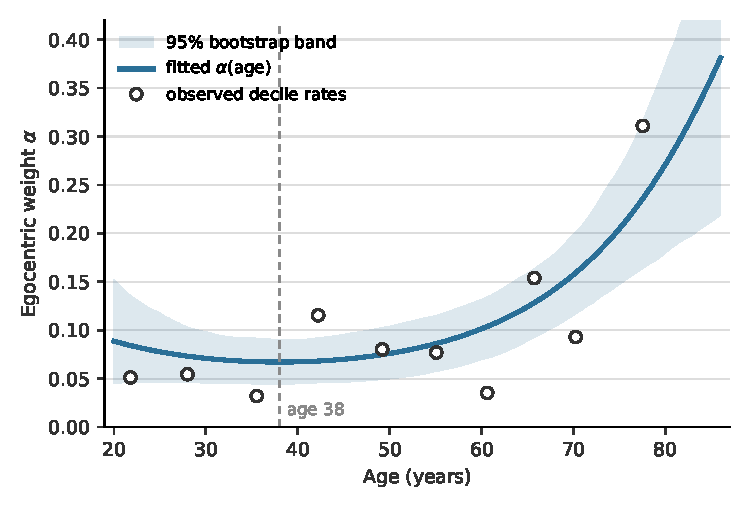
\includegraphics[width=.8\linewidth]{figures/curve.pdf}
  \caption{Fitted egocentric weight $\alpha(\mathrm{age})$ (line) with its 95\%
  band from 1{,}000 participant-level bootstrap resamples (deterministic replay
  of the protocol's seeded bootstrap), observed pooled egocentric rates by age
  decile (open circles; $\approx$26 participants each), and the fitted minimum
  at age 38.0 (dashed line). All values are conditional on the
  probability-matching response rule; under the argmax-plus-lapse reading every
  value doubles ($\varepsilon = 2\alpha$; Proposition~\ref{prop:equivalence}).}
  \label{fig:curve}
\end{figure}

\subsection{Held-out participant prediction}\label{sec:cv}

The age-dependent model produced a positive held-out log-likelihood difference
over the fitted constant-$\alpha$ model in \textbf{20 of 20} repeats (mean
$+9.35$, median $+9.56$, range $[+7.06, +10.90]$), meeting the prespecified
stability rule R2. The per-participant mean out-of-fold difference was
$+0.035$, positive for 65.2\% of participants (descriptive summaries; no
$p$-value is attached, as repeats are correlated). The overall outcome category
is \textbf{Meets prespecified robustness criteria}. The bootstrap completed
1000/1000 refits without failures.

\subsection{A prespecified model failure}\label{sec:t2}

T1 passed: the observed pooled egocentric rate at ages 73--86 ($0.290$) fell
within the model's 95\% predictive interval $[0.156, 0.358]$. \textbf{T2 failed
beyond the 99\% interval:} 18 participants aged 20--37 made exactly one
egocentric error, against a predictive interval of $[1, 11]$. The fitted
hierarchy, which accounts for the age trend and for heavy individual
heterogeneity ($\kappa \approx 1.4$), cannot reproduce the observed excess of
single-error young adults. We report this as a result: a single age-varying
mixture process, with this response rule, does not fully account for errors at
both ends of the adult age range.

\subsection{Sensitivity analyses}\label{sec:sensitivity}

The estimand was stable in every prespecified probe: fine grids,
$\dalpha = +0.1270$ (unchanged to four decimals); IQ cutoffs from none to 80,
\dalpha{} between $+0.1225$ and $+0.1270$; full leave-one-participant-out,
maximum $|\Delta\dalpha| = 0.0099$ ($\approx$8\% of the estimate, below the
prespecified flag); leave-one-trial-position-out, maximum
$|\Delta\dalpha| = 0.0100$ (with the recorded caveat that trial position may
conflate item identity in this dataset).

% =========================================================================
\section{Discussion}\label{sec:discussion}
% TODO (FL): paragraphs 1-7 per paper/OUTLINE.md scaffold.

% =========================================================================
\section*{Data and Code Availability}
All analysis code, the frozen protocol with dated addenda, and the verbatim
execution log are public at \repo{} (key commits: freeze \texttt{e09d306};
amendments \texttt{a8de96b}, \texttt{be30e90}; implementation \texttt{63943b1};
results \texttt{9764283}). The dataset is \citet{bradford2023}'s open data at
\url{https://osf.io/2epsu/}, cited rather than redistributed.

\section*{AI Assistance Disclosure}
% [Per venue policy; see OUTLINE.md for the division-of-labor wording.]

\section*{Acknowledgments}
We thank Bradford, Brunsdon and Ferguson for publishing their data and code.

\bibliographystyle{apalike}
\bibliography{references}

\appendix
\section{Protocol deviations and addenda}\label{app:addenda}
% [Addenda 1-2 verbatim, or reference to the public protocol file.]

\end{document}
